 \subsubsection{UC10 - Gestione veicoli}
  \begin{figure}[H]
 	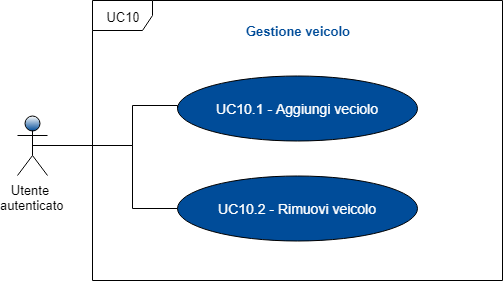
\includegraphics[width=10cm]{res/images/UC10Gestioneveicolo.png}
 	\centering
 	\caption{UC10 - Gestione Veicoli}
 \end{figure}
 \begin{itemize}
 	\item \textbf{Attori Primari}: utente autenticato;
 	\item \textbf{Descrizione}: l'utente ha una panoramica dei veicoli che ha inserito visualizzando solo poche cose riguardanti il mezzo e ha la possibilità di:
 	\begin{itemize}
 		\item aggiungere un veicolo [UC10.1];
 		\item visualizzare i dettagli del veicolo [UC10.2].
 	\end{itemize}
 	\item \textbf{Precondizione}: l'utente accede al fragment\glosp per la gestione dei veicoli;
 	\item \textbf{Postcondizione}: l'utente visualizza le informazioni relative ai propri veicoli, con le eventuali operazioni disponibili su ognuno di essi.
 \end{itemize}
 \subsubsection{UC10.1 - Aggiungi veicolo}
 \begin{itemize}
 	\item \textbf{Attori Primari}: utente autenticato;
 	\item \textbf{Descrizione}: l'utente può aggiungere un mezzo di trasporto al proprio parco macchine;
 	\item \textbf{Scenario principale}: l'utente aggiunge un veicolo compilando gli appositi campi obbligatori, ovvero:
 	\begin{itemize}
 		\item inserimento immagine veicolo [UC10.1.1];
 		\item inserimento marca veicolo [UC10.1.2];
 		\item inserimento modello veicolo [UC10.1.3];
 		\item inserimento anno d'immatricolazione veicolo [UC10.1.4].
 	\end{itemize}
 	e successivamente salverà il nuovo veicolo confermando i campi appena inseriti;
 	\item \textbf{Precondizione}: l'utente ha inserito correttamente tutti i campi necessari;
 	\item \textbf{Postcondizione}: il nuovo veicolo viene aggiunto ai veicoli posseduti.
 \end{itemize}
\begin{figure}[H]
	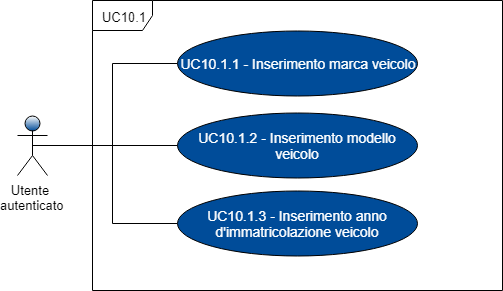
\includegraphics[width=10cm]{res/images/UC10-1Aggiungiveicolo.png}
	\centering
	\caption{UC10.1 - Aggiungi veicolo}
\end{figure}
\subsubsection{UC10.1.1 - Inserimento immagine veicolo}
\begin{itemize}
	\item \textbf{Attori Primari}: utente autenticato;
	\item \textbf{Descrizione}: al fine di portare a termine il processo di inserimento di un nuovo veicolo l'utente deve inserire un'immagine del proprio mezzo, campo ritenuto obbligatorio; 
	\item \textbf{Scenario principale}: l'utente preme il pulsante relativo all'inserimento dell'immagine del veicolo;	
	\item \textbf{Precondizione}: l'applicazione ha reso disponibile il bottone per l'inserimento dell'immagine del veicolo;
	\item \textbf{Postcondizione}: l'utente ha inserito correttamente l'immagine del veicolo.
\end{itemize}
\subsubsection{UC10.1.2 - Inserimento marca veicolo}
\begin{itemize}
	\item \textbf{Attori Primari}: utente autenticato;
	\item \textbf{Descrizione}: al fine di portare a termine il processo di inserimento di un nuovo veicolo l'utente deve inserire la marca, campo ritenuto obbligatorio;
	\item \textbf{Scenario principale}: l'utente compila il campo relativo alla marca del veicolo;	
	\item \textbf{Precondizione}: l'applicazione ha reso disponibile il campo per l'inserimento della marca del veicolo;
	\item \textbf{Postcondizione}: l'utente ha compilato il campo con la marca.	
\end{itemize}

\subsubsection{UC10.1.3 - Inserimento modello veicolo}
\begin{itemize}
	\item \textbf{Attori Primari}: utente autenticato;
	\item \textbf{Descrizione}: al fine di portare a termine il processo di inserimento di un nuovo veicolo l'utente deve inserire il modello, campo ritenuto obbligatorio;
	\item \textbf{Scenario principale}: l'utente compila il campo relativo alla marca del veicolo;	
	\item \textbf{Precondizione}: l'applicazione ha reso disponibile il campo per l'inserimento il modello del veicolo;
	\item \textbf{Postcondizione}: l'utente ha compilato il campo con il modello.	
\end{itemize}
\subsubsection{UC10.1.4 - Inserimento anno d'immatricolazione veicolo}
\begin{itemize}
	\item \textbf{Attori Primari}: utente autenticato;
	\item \textbf{Descrizione}: al fine di portare a termine il processo di inserimento di un nuovo veicolo l'utente deve inserire l'anno di immatricolazione, campo ritenuto obbligatorio;
	\item \textbf{Scenario principale}: l'utente compila il campo relativo all'anno d'immatricolazione del veicolo;	
	\item \textbf{Precondizione}: l'applicazione ha reso disponibile il campo per l'inserimento dell'anno d'immatricolazione del veicolo;
	\item \textbf{Postcondizione}: l'utente ha compilato il campo con l'anno d'immatricolazione.	
\end{itemize}

%\subsubsection{UC10.1.4 - Invio dati veicolo}
%\begin{itemize}
%	\item \textbf{Attori Primari}: utente autenticato;
%	\item \textbf{Descrizione}: l'utente preme il pulsante per la conferma e l'invio dei dati del veicolo;
%	\item \textbf{Scenario principale}: l'utente preme il pulsante di verifica ed invio dei dati;	
%	\item \textbf{Precondizione}: i campi dati necessari per l'inserimento di un veicolo sono compilabili. È presente il pulsante per la conferma dei dati;
%	\item \textbf{Postcondizione}: il nuovo veicolo viene inserito e l'utente potrà visualizzarlo nel proprio parco macchine.
%\end{itemize}
\subsubsection{UC10.2 - Visualizza dettagli veicolo}
\begin{itemize}
	\item \textbf{Attori Primari}: utente autenticato;
	\item \textbf{Descrizione}: l'utente autenticato, per ogni veicolo, può visualizzare in dettaglio le seguenti informazioni:
	\begin{itemize}
		\item marca;
		\item modello;
		\item anno di immatricolazione;
		\item rating.
	\end{itemize}
	E ha la possibilità di rimuovere il veicolo [UC10.2.1];
	\item \textbf{Scenario principale}: l'utente visualizza i dati di dettaglio del veicolo;
	\item \textbf{Precondizione}: l'utente autenticato visualizza i dettagli del veicolo;
	\item \textbf{Postcondizione}: l'utente autenticato ha visualizzato i dettagli del veicolo.
\end{itemize}
\begin{figure}[H]
	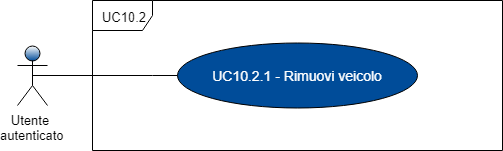
\includegraphics[width=10cm]{res/images/UC10-2Dettagliveicolo.png}
	\centering
	\caption{UC10.2 - Visualizza dettagli veicolo}
\end{figure}

\subsubsection{UC10.2.1 - Rimuovi veicolo}
\begin{itemize}
	\item \textbf{Attori Primari}: utente autenticato;
	\item \textbf{Descrizione}: l'utente può rimuovere un mezzo di trasporto dal proprio parco macchine;
	\item \textbf{Scenario principale}: l'utente, dopo aver selezionato il veicolo da visualizzare, può rimuoverlo dal proprio parco macchine attraverso l'apposito pulsante;
	\item \textbf{Precondizione}: l'applicazione mostra all'utente i propri veicoli e ne permette la selezione;
	\item \textbf{Postcondizione}: il veicolo selezionato viene rimosso dal parco macchine.
\end{itemize}